\graphicspath{{Chapter_3_-_Thermodynamic_components/Images/}}
\chapter{Thermodynamic components}
\quad\, In the beginning of the previous chapter, it has been mention that the Brayton cycle composed of several components that are more or less complex. The behavior of these components, which is required to realized the study the global system, is based on the thermodynamic notions that have be introduce all along the past lines.

This chapter will be focused on the description of those components. For each of them, it will be provided a state of the art followed by the concepts or principles that will be used during this work. 
\section{Turbomachines}
\quad\, The first family of components to be studied is the turbomachines. The machines owning to this family are ones "that exchange energy between the
fluid traversing it and mechanical energy supplied to or extracted from the machine" \cite{Hillewaert2019}. Those machines are \textbf{rotating} machines and, based on the compressible nature of the fluid, two categories can be created.
This subsection will swept the two categories but will mainly focused on the machines exchanging energy with \textbf{compressible} flow.

\subsection{Incompressible flow}
\quad\, The first category of flow to be considered is the incompressible flow. This type of flow is characterized by a constant density over the distance. An example of incompressible fluid is the water.

Among the machine exchanging energy with such type of fluid, there are pumps which are designed to raise the height or total hydraulic energy $h$ of the fluid. The variation of the height of the fluid is similar to its enthalpy variation. Thus, the power output  $\dot{W}_p$ developed by the pump can be expressed as given in relation (\ref{eq:C3_Ppump})
\begin{equation}
\dot{W}_{p,a-b} = \dot{m}\cdot (h_a - h_b)=\dot{m}\cdot\Delta h_p \label{eq:C3_Ppump}
\end{equation}
considering that the transformation makes the system going from state \textbf{a} to state \textbf{b}.

If the consumed power of the pump is $\dot{W}_{e,a-b}$, its global efficiency $\eta_p$ is equal to the ratio
\begin{equation}
\eta_p = \frac{\dot{W}_{p,a-b}}{\dot{W}_{e,a-b}}\label{eq:C3_Etapump}
\end{equation}
\subsubsection{Characteristic maps}
\quad\, It has be shown that the power output and the global efficiency of the pump are functions of the height variation and the flow rate of the fluid. When operating a pump, it can be useful to know how this height variation will vary with respect to the flow rate and the rotational speed of the pump shaft. The knowledge of these two parameters allows to fully characterized the pump.

Considering the volumetric flow rate $Q_p$ (m$^3$/s) and the rotational speed $\Omega$, the two following relations (\ref{eq:C3_DHp}) and (\ref{eq:C3_Pe}) can be derived.
\begin{align}
\setstretch{1}
\Delta h_p &= f(Q_p, \Omega)\label{eq:C3_DHp}\\
\dot{W}_e &= f(Q_p, \Omega)\label{eq:C3_Pe}
\end{align}
Those relations will be called characteristic or performance Map and are determined \textbf{experimentally}. An example of such map is given on Figure \ref{fig:C3_MapPump}.
\begin{figure}[h]
\centering
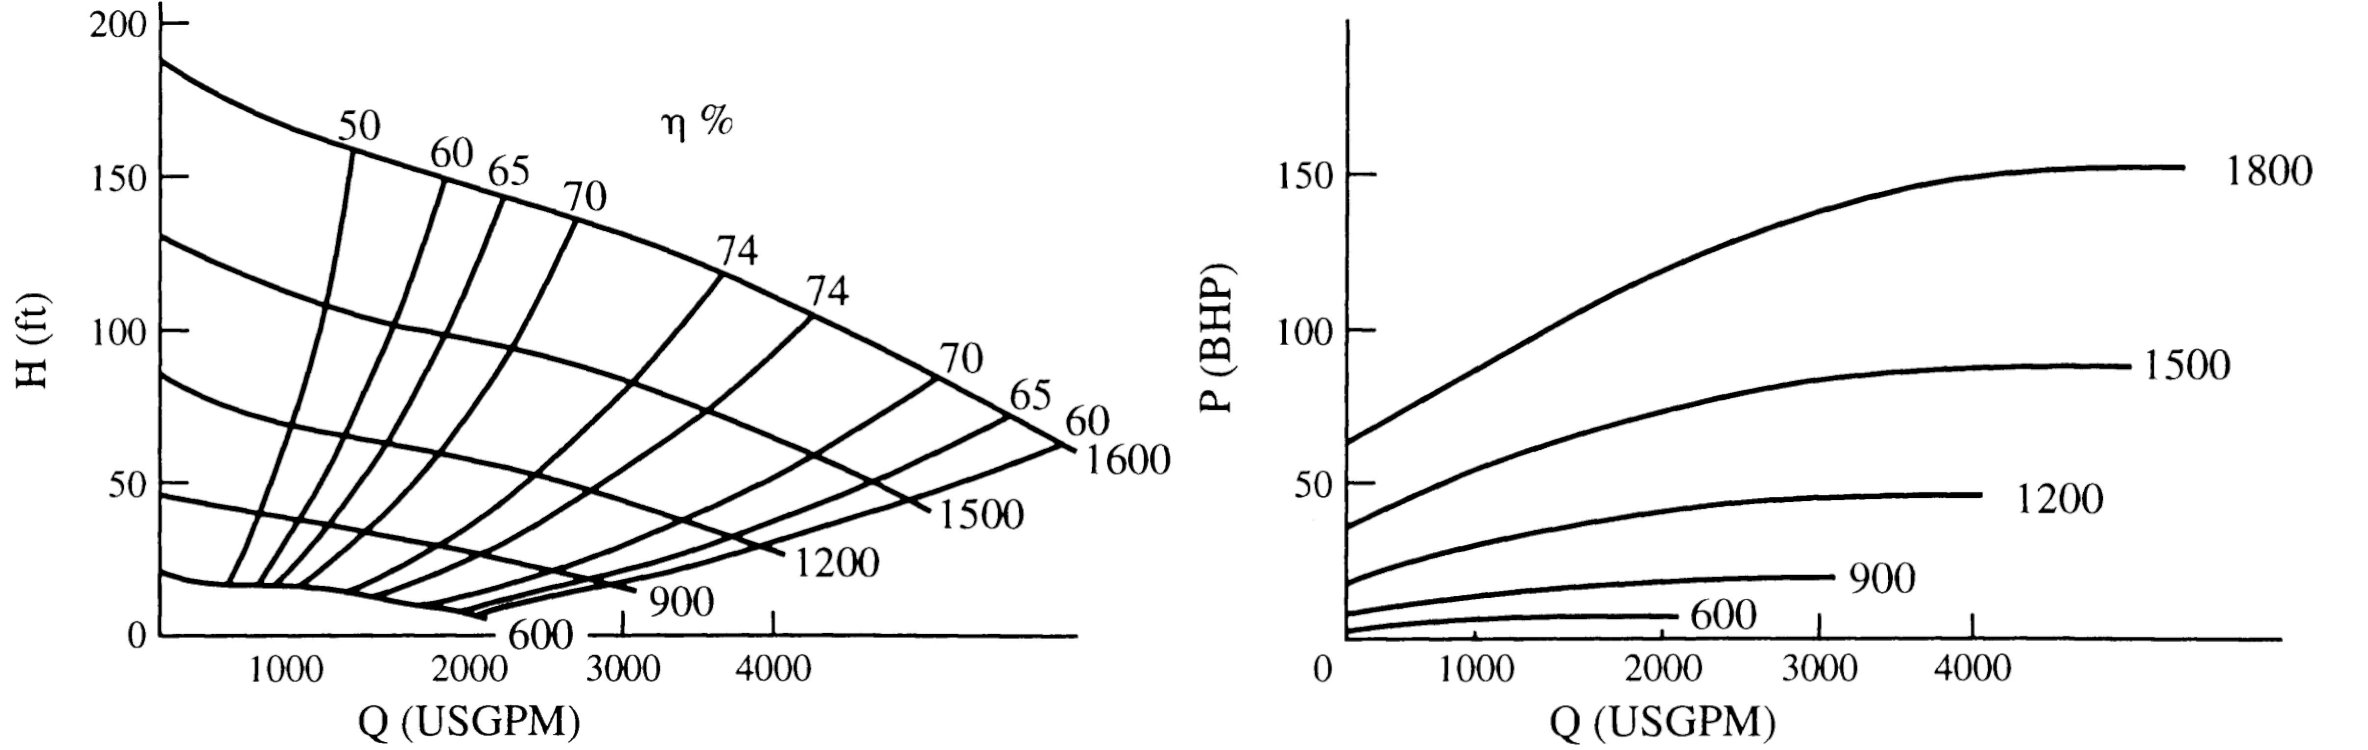
\includegraphics[width=0.8\textwidth]{char_map_pump.png}
\caption{Characteristic maps of a pump \citep{Hillewaert2019}}
\label{fig:C3_MapPump}
\end{figure}
\subsubsection{Similarity}
\quad\, When considering incompressible flow, it is possible to extrapolate from a known operating point a infinity of similar operating points. Indeed, There exist relationships which provides with enough accuracy the change of flow rate $Q$ and height variation $\Delta H$ when the rotational speed goes from $\Omega_1$ to $\Omega_2$. It can be demonstrate that the flow rate evolves linearly with the rotation speed, and that the height variation is a quadratic function of $\Omega$.
\begin{align}
\setstretch{1}
Q_2 &= Q_1\cdot\frac{\Omega_2}{\Omega_1} \label{eq:C3_Qsim}\\
\Delta h_2 &= \Delta h_1\cdot\left(\frac{\Omega_2}{\Omega_1}\right)^2 \label{eq:C3_DHsim}
\end{align} 
These relations are really useful to extrapolate the performance maps of a pump. Similar relations can be deduced considering the variation of the radius of the pump.

One important property to notice is that all the dimensionless variables (e.g. the efficiency) are kept constant for all the different similar operational points. This is a valuable property which will be very useful for the future developments of the thesis.
\subsubsection{Types of pumps}
\quad\, Now that the exterior characteristics of the pumps have been defined, it is interesting to have at least a brief idea about how the pump is constructed. Without entering into detailed\footnote{see the section 4.3 and 4.4 of the course \citep{Hillewaert2019}}, there are two types of pumps.

The first type to be considered is the centrifugal pumps designed to provide a high heat for a low flow rate. Those pumps are characterized by an axial inflow and a radial outflow. The Figure \ref{fig:C3_centri_pump} shows a schematic of a centrifugal pumps.
\begin{figure}[h]
\centering
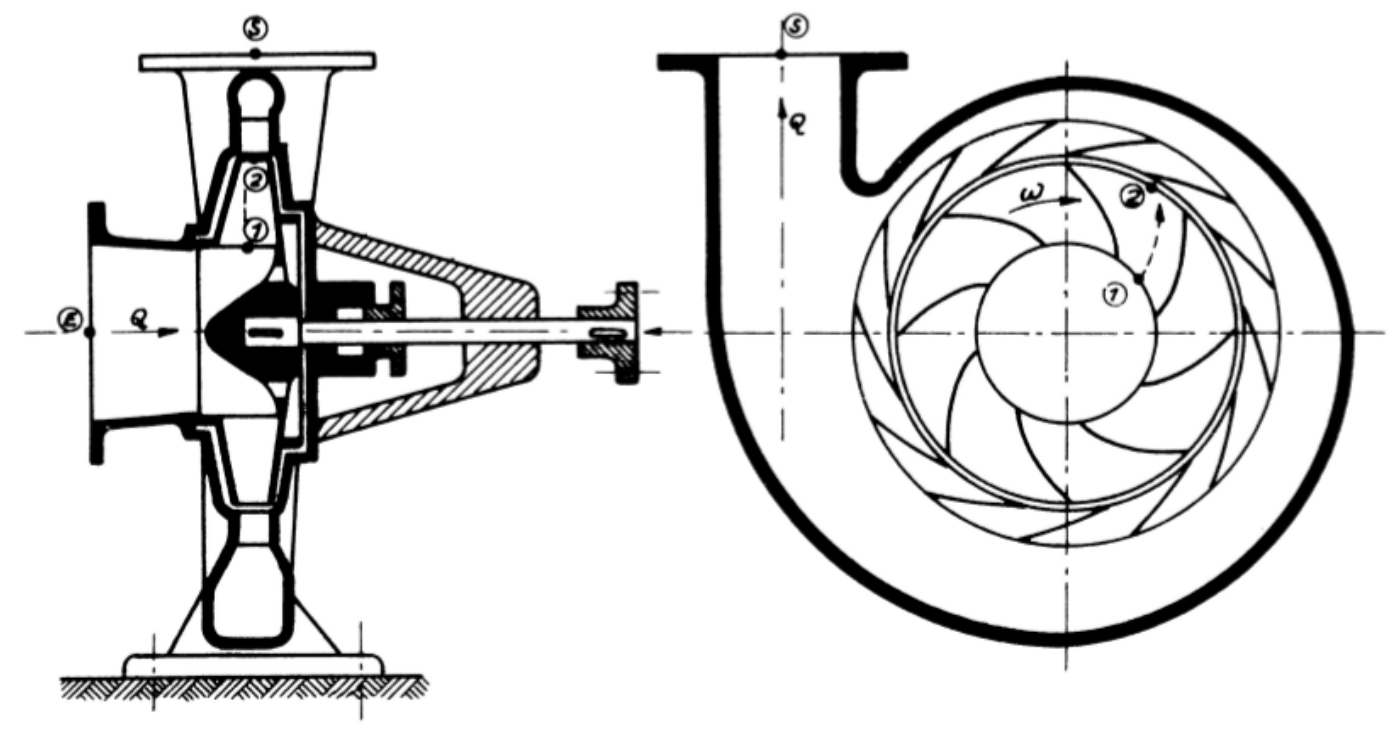
\includegraphics[width=0.4\textwidth]{centri_pump.png}
\caption{Centrifugal pump \citep{Hillewaert2019}}
\label{fig:C3_centri_pump}
\end{figure}

Basically, the centrifugal pump can be decomposed into two parts (for the most simple device). The first  part is the rotating impeller that will convert and transfer the mechanical energy to the fluid. Behind the impeller will be placed the volute (right picture of Figure \ref{fig:C3_centri_pump}) that collects the flow to bring it to the outlet of the pump.\newpage

The second type of pump are the axial pumps which are, in opposition with the centrifugal pumps, designed to deliver low head for high flow rates. Such pumps is illustrated on Figure \ref{fig:C3_axial_pump}. 
\begin{figure}[h!]
\centering
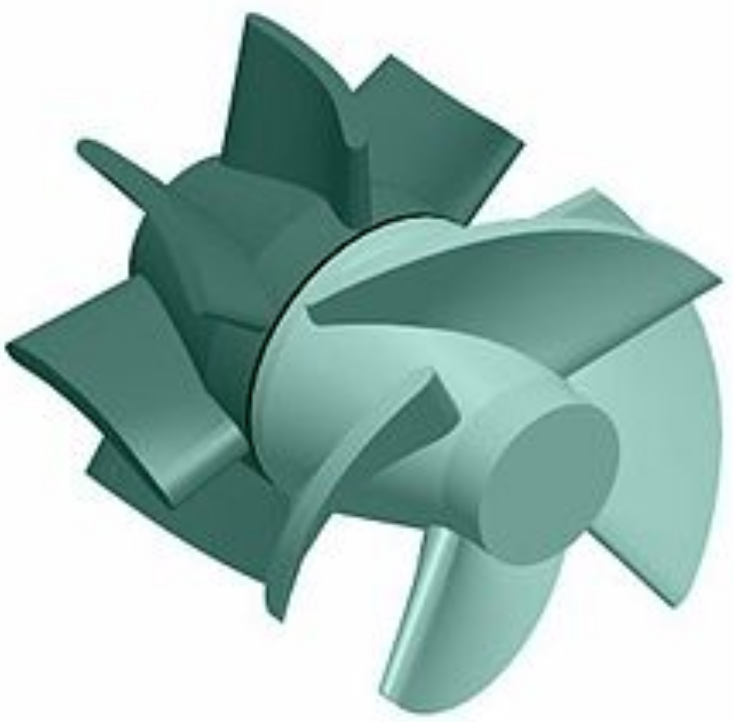
\includegraphics[width=0.25\textwidth]{axial_pump.png}
\caption{Axial pump \citep{Hillewaert2019}}
\label{fig:C3_axial_pump}
\end{figure}

The main two parts of an axial pumps are the rotor (the rotating part) that will increase the height of the fluid followed by a diffusor which "recuperates the kinetic energy at the exit of the rotor"\citep{Hillewaert2019}.

\subsection{Compressible flow}
\quad\, The previous subsection introduced the pump which is a turbomachine design to increase the energy of the incompressible fluid passing through it. However, this type of machine cannot deals with compressible flow for which the density can vary over the distance. For instance, the air is a compressible fluid. 

The behavior of the compressible flow is more complex to describe compared to incompressible flow. Indeed, "compressible flow is characterized by the propagation of acoustic waves"\citep{Hillewaert2019}.   This part of the section about turbomachines will only focused on the very main principles required for the good understanding of this work.

\subsubsection{Static and total quantities}
\quad\, As it has be partly reveal in the previous lines, the flow characteristics are dependent on its velocity. The study of compressible flow did lead to the distinction between the static and total quantities. 

The static quantities are state variables (e.g. temperature, pressure,...) that are independent of the flow velocity. As for the total quantities, these are dependent of the flow velocity $V$. For instance, the total enthalpy is given by
$$
h^0 = h + \frac{1}{2}\cdot v^2.
$$
where the total quantity is identified by the superscript "0".

The total enthalpy can be defined as "the static enthalpy obtained when the gas is brought adiabatically to a halt"\citep{Hillewaert2019}.


\subsubsection{Conservation of the total enthalpy and rothalpy}
\quad\, For an adiabatic transformation without viscous work, the total enthalpy is conserved between the initial state and the final state.
\begin{equation}
\dot{m}\cdot h_1^0 = \dot{m} h_2^0 \label{eq:C3_hcons}
\end{equation}
which can be reduced to $h_1^0 = h_2^0$ if we supposed that the transformation is performed without any leakages. The states $1$ and $2$ are associated to the orthogonal boundaries to the flow of the selected control volume delimiting the studied system. 

Now, considering a rotating system (e.g. a rotor), the variation of the total enthalpy can be obtained by considering the modified Euler equation of turbomachinery
\begin{equation}
h_2^0 - h_1^0 = \frac{1}{2}\cdot \left(v_2^2 - v_1^2\right) - \frac{1}{2}\cdot \left(wr_2^2 - wr_1^2\right) + \frac{1}{2}\cdot \left(ur_2^2 - ur_1^2\right)\label{eq:C3_Euler}
\end{equation}
where $v$ is the average flow velocity through a surface, $wr$ is the velocity of the flow relative to the rotor and $ur$ is the velocity of the rotor. Defined the total rothalpy as being 
\begin{equation}
i^0 = h^0 + \frac{1}{2}\cdot wr^2 - \frac{1}{2}\cdot ur^2 
\end{equation}
It is obtained from the Euler equation (\ref{eq:C3_Euler}) that the total rothalpy is conserved through the transformation.
\begin{equation}
i_1^0 = i_2^0 \label{eq:C3_icons}
\end{equation}
\subsubsection{Mach number}
The Mach number $M$ is defined as being the ratio between the velocity $V$ and the sound speed $a$.
\begin{equation}
M = \frac{V}{a} \label{eq:C3_Mach}
\end{equation}
The Mach number $M$ is a dimensionless variable that gives an image of the compressible effects of the flow. Thus, one criteria for the determination of similar operational points is to keep constant the Mach number.

Using the Mach number allows to obtain formulas to compute the total quantities base the static ones. By considering first the total temperature, it can be found
\begin{equation}
T^0 = T + \frac{V^2}{2\cdot c_p} = T\cdot\left(1 + \frac{V^2}{2\cdot c_p\cdot T}\right)\label{eq:C3_TT0_1}
\end{equation}
For an isentropic process, it can be demonstrate that the speed of sound $a=k\cdot r\dot T$. Thus, the equation (\ref{eq:C3_TT0_1}) becomes
\begin{equation}
T^0 = T\cdot\left(1 + \frac{k-1}{2}\cdot M^2\right) = T\cdot f(M) \label{eq:C3_TT0}
\end{equation}
Using the equations \ref{eq:C2_isrel}) and the definition of the function $f(M)$, the relations linking the static to the total pressure, density and speed of sound can be obtained as well.
\begin{align}
\setstretch{1}
P^0 &= P\cdot f(M)^\frac{k}{k-1}\label{eq:C3_PP0}\\
\rho^0 &= \rho\cdot f(M)^\frac{1}{k-1}\label{eq:C3_rhorho0}\\
a^0 &= a\sqrt{f(M)} \label{eq:C3_aa0}
\end{align}
\subsubsection{Performance maps}
\quad\, As for the turbomachines exchanging energy with incompressible flows, the one studied here can be fully characterized knowing two independents operating parameters. Usually, the four parameters used for the drawing of the maps are
\begin{itemize}
\setstretch{1}
\item $\dot{m}_c$ (kg/s or lbs/min): It is the corrected mass flow, it is defined as follows
\begin{equation}
\dot{m}_c = \dot{m}\cdot \sqrt{\frac{T}{T_{ref}}}\cdot\left(\frac{P_{ref}}{P}\right)
\end{equation}
with $T_{ref}$ and $P_{ref}$ being the reference temperature and pressure (all quantities being static).

\item $\Omega$ (rpm): It is the rotational speed of the turbomachine shaft. 

\item $\Pi$ (-): It is the pressure ratio between the inlet and the outlet of the turbomachines. If the turbomachines is compressing the flow, the ratio is reverse to keep it greater than one.

\item $\eta$ (-): It is the isentropic efficiency of the machine.
\end{itemize} 
\subsection{Gas compressor}
\quad\, The gas compressor is designed to raise the pressure of a compressible gas. 